\section{Overview}
The shortcomings of the existing work inspire us to design a new tool to detect
and quantify information leakage vulnerabilities in binaries. The tool has three
steps. First, we run the target program with the concrete input 
(sensitive information) under the dynamic binary instrumentation (DBI) frameworks
to collect the execution traces. After that, we run the symbolic execution 
to capture the fined-grained semantic information of each secret-dependent 
control-flow transfers and data-accesses. 
Finally we run the Markov Chain Monte Carlo (MCMC) to estimate the 
information leakage. 

\begin{figure*}[ht]
    \centering
    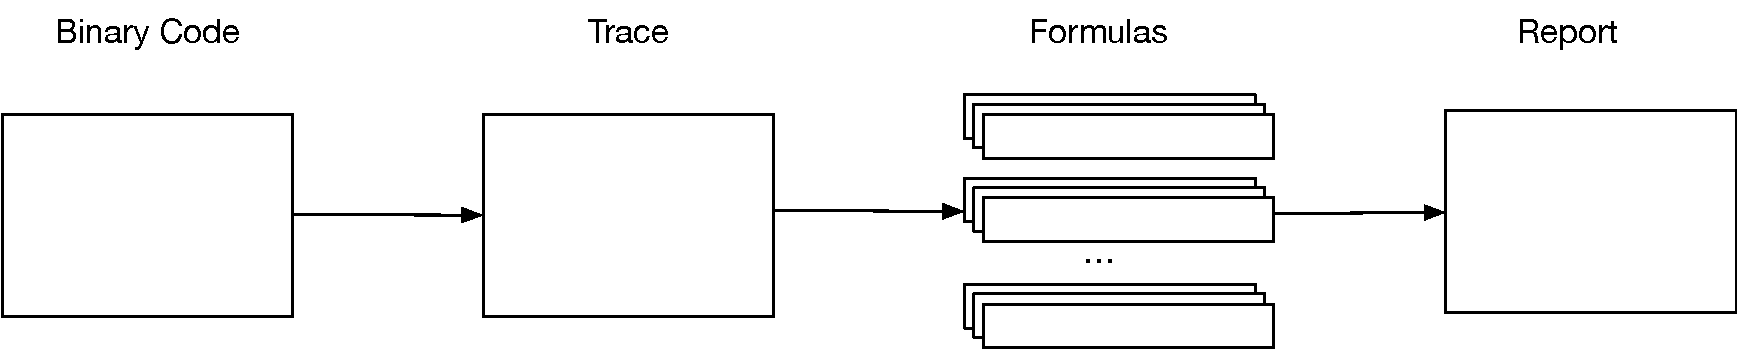
\includegraphics[width=\columnwidth]{./figures/workflow.pdf}
    \caption{The workflow of \tool{}}
    \label{fig:Test}
\end{figure*}

\begin{enumerate}
    \item \textit{Execution trace generation.} The design goal of \tool\ is to
    estimate the information leakage as precisely as possible. Therefore,
    we sacrifice the soundness for the precision in terms of program analysis.
    Previous works~\cite{203878,217537} have demonstrated the effectiveness of the
    dynamic program analysis. We run the target binary under the dynamic binary
    instrumentation (DBI) to record the execution trace and the runtime information.
    \item \textit{Instruction level symbolic execution.} We model the 
    attacker's observation about the side-channel vulnerabilities with math
    formula. Each formula capture the fined-grained information between the input secrets
    and the leakage site. For the consideration of precision and performance, 
    we remove the intermediate language(IR) layer of the symbolic execution. 
    Also, the engine only symbolically execute the instruction that might be affected the
    input key. The above design significantly reduces the overhead of the symbolic
    execution, which make the tool scales to real-world programs.
    \item \textit{Leakage estimation.} We transfer the information leakage quantification
    problem into the problem of counting the number of assignments that satisfy the formulas
    which models the observations from attacker. We propose a markov monte carlo method to 
    estimate the number of satisfied solutions. With the help of Chebyshev's Inequality,
    we also give the an error estimate with the probability.
\end{enumerate}
